\label{chap:conclusao}

De acordo com o desenvolvido no capítulo \ref{chap:analise}, com
as tabelas \ref{tab:prototipo-vs-cluster} e \ref{tab:prototipo-analise},
contrasta a homogeneidade dos protótipo 2 e 3 à heterogeneidade do
protótipo 1. À primeira vista, percebe-se que os três protótipos possuem
proporções da população muito parecidas, entretanto há uma grande
diferença entre o protótipo 1, heterogêneo, com os demais protótipos.
Isto é, a possibilidade de uma campanha publicitária informativa unida
a transformativas que possibilitarão, se escolhido o protótipo 1,
abranger também os clusters \nomeCc{} e \nomeCb{}, dado que pela
própria heterogeneidade do protótipo 1, certas propagandas que apelam
para determinadas características do protótipo podem aumentar a aceitação
de uma campanha baseada neste protótipo.

\begin{table}
\begin{centering}
\begin{tabular}{c|>{\centering}p{0.28\textwidth}|>{\centering}p{0.28\textwidth}|>{\centering}p{0.28\textwidth}}
\hline 
 & Protótipo 1 & Protótipo 2 & Protótipo 3\tabularnewline
\hline 
Bom & Preferido entre \nomeCa{} e \nomeCd{}. & Amplamente preferido pelo cluster dos \nomeCc{}. & Amplamente preferido pelos \nomeCb{}, focados em Imagem.\tabularnewline
\hline 
Ruim & Somente uma estratégia de marketing não é suficiente, dada a sua heterogeneidade
e várias afinidades. & Difícil para a publicidade porque se mostra indiferente a carros.
Importam-se apenas com o preço. & Uma campanha publicitária em Imagem somente não gera interesse de
outros clusters.\tabularnewline
\hline 
\end{tabular}
\par\end{centering}
\caption{\label{tab:prototipo-analise}Vantagens e desvantagens por protótipos.}
\end{table}

\begin{figure}
\begin{centering}
\subfloat[\label{fig:prototipo-familia}Conforto,
espaço e filhos.]{\begin{centering}
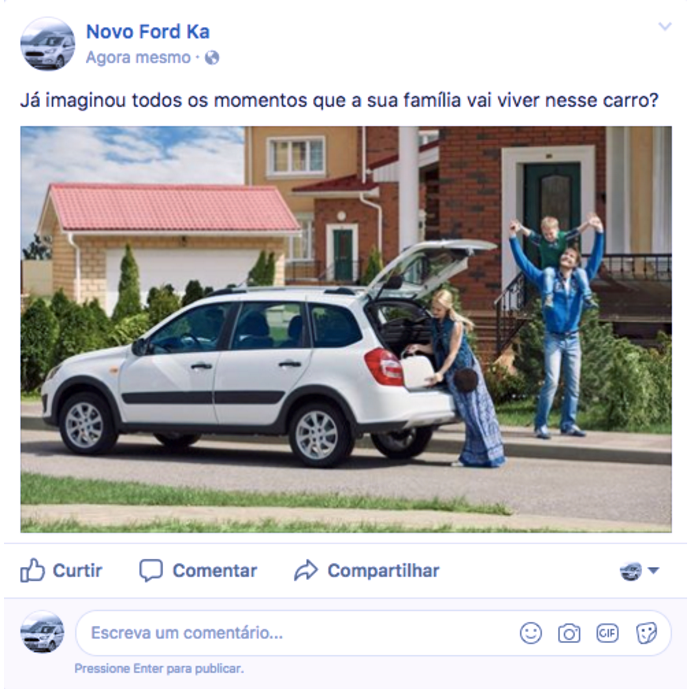
\includegraphics[height=0.30\textheight]{Imagens/p1_familia}
\par\end{centering}
}\subfloat[\label{fig:prototipo-versatil}Aborda o efeito versátil do carro.]{\begin{centering}
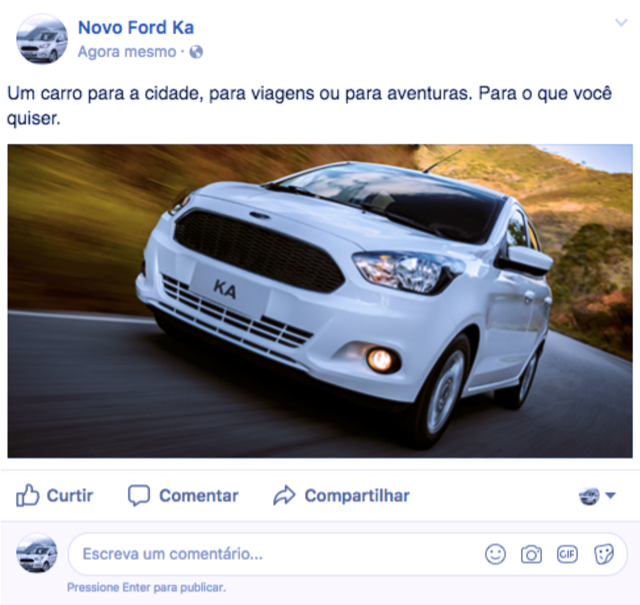
\includegraphics[height=0.30\textheight]{Imagens/p1_prototipo}
\par\end{centering}
}
\par\end{centering}
\caption{Peças ilustrativas de uma campanha em formato carrossel, unindo marketing informativo, voltado a Utilitário, ao transformativo (Imagem, Preço, Filhos, Gênero...).}
\end{figure}


Por exemplo, se uma campanha publicitária apelar de maneira informativa
e transformativa para os aspectos de Imagem e Utilitário do carro,
é possível abranger os clusters mencionados anteriormente, sustentando
assim uma aceitação maior por parte da população. Ou seja, escolhe-se
a versatilidade do protótipo 1, numa eventual campanha publicitária
como elemento.

\begin{figure}
\begin{centering}
\subfloat[\label{fig:painel-cambio}Acabamento e câmbio.]{\begin{centering}
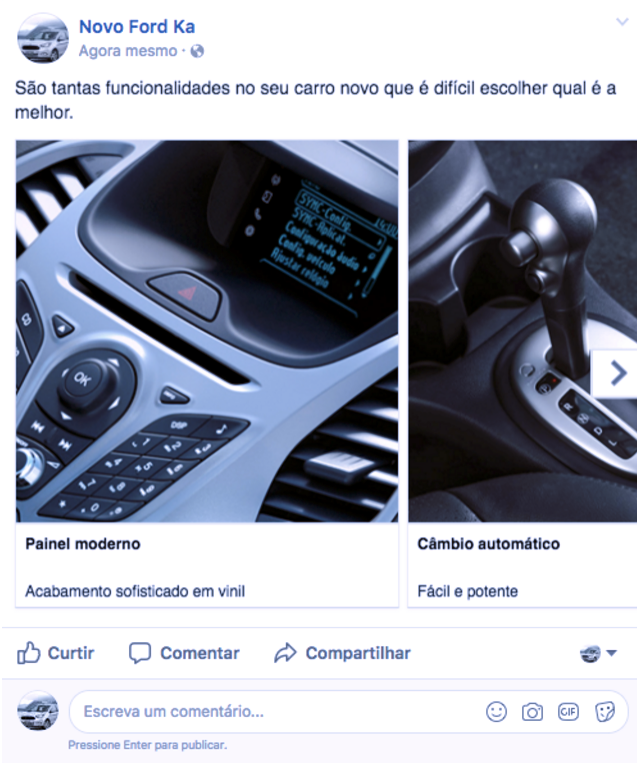
\includegraphics[height=0.37\textheight]{Imagens/p1_interior}
\par\end{centering}
}\subfloat[\label{fig:ar}Ar-condicionado.]{\begin{centering}
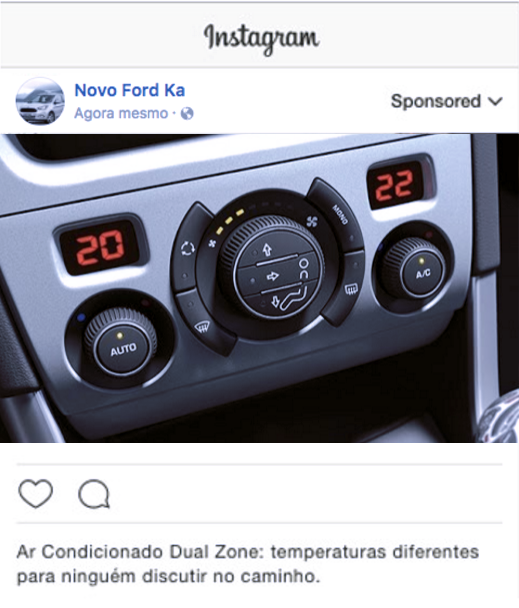
\includegraphics[height=0.37\textheight]{Imagens/p1_interior_painel}
\par\end{centering}
}
\par\end{centering}
\caption{Peças multifuncionais para demonstrando o interior do carro, aliando Imagem a Utilitário para o protótipo 1, voltado a um público heterogêneo.}
\end{figure}


\section{Campanha Publicitária: Protótipo 1}

Com base nas características analisadas dos grupos \nomeCa{} e \nomeCd{}
será feita uma combinação de campanhas publicitárias: para os \nomeCa{},
uma campanha transformativa mesclando os três atributos: Imagem, Utilitário
e Preço. Para os \nomeCd{}, uma campanha ressaltando o carro como
utilitário. Por se tratar de dois grupos diferentes vamos destacar
multifuncionalidade, tecnologia, versatilidade e conforto.

É possível uma campanh que foque nas seguintes características: confortável
e espaçoso. O público-alvo seriam os \nomeCd{} que preferem carros
como bens utilitários, destacando o porta-malas espaçoso para a família.
Os \nomeCd{} são formados predominantemente por mulheres com filhos,
por isso o destaque a família, na figura \ref{fig:prototipo-familia}.

A campanha com formato em carrossel irá abordar a característica de
multifuncionalidade. A publicidade tem foco nos \nomeCa{} combinando
funcionalidades (Utilitário) que valorizem o carro (Preço) e que tragam
mais sofisticação (Imagem), como vê-se nas figuras \ref{fig:painel-cambio}
e \ref{fig:ar}.

Finalmente, a figura \ref{fig:prototipo-versatil} seria veiculada
em formato vídeo, tanto em Facebook quanto na televisão. Destaca a
versatilidade do Ford Ka\texttrademark, valorizando o fato de ser
um carro potente (Utilitário) e ainda assim econômico (Preço). Em
televisão, dá-se preferência é por intervalos de jogos de futebol
buscando atingir um público predominantemente masculino que gosta
de esportes e aventuras. 
